\documentclass[10pt, a4paper]{article}

\usepackage[a4paper, top=0.5cm, bottom=0.5cm, left=0.5cm, right=0.5cm, landscape]{geometry}
\usepackage{mathtools}
\usepackage{amsfonts}
\usepackage{multicol}
\usepackage{setspace}
\usepackage{graphicx}
\usepackage[dvipsnames]{xcolor}



\author{Zachary Chua Yan Ern}
\date{22 September 2021}
\setstretch{1.25}

\newcommand{\highlight}[1]{{\color{red}\textbf{#1}}}
\newcommand{\blue}[1]{{\color{MidnightBlue}#1}}
\newcommand{\red}[1]{{\color{red}#1}}
\newcommand{\green}[1]{{\color{ForestGreen}#1}}

\begin{document}
	\scriptsize %tiny
	\setlength\parindent{0pt}
	\setlength{\columnseprule}{0.1pt}
	
	\begin{center}
		{\large CS2105 CheatSheet}\\
		by Zachary Chua
	\end{center}
	
	\begin{multicols*}{3}
		{\normalsize\textbf{Internet}}\\
		- The Internet is a network of connected computing devices\\
		- Devices are known as \highlight{hosts} or \highlight{end systems}\\
		- Hosts run network applications (like browsers) and communicate over links\\
		
		\textbf{Network Edge (Access Network)}\\
		- Hosts access the Internet through \highlight{access network}\\
		- eg Home/ Institute access networks\\
		
		\textbf{Wireless Access Network}\\
		1. Wireless LAN (WIFI): Short range (100 ft)\\
		2. Wide-area wireless access (3G/ 4G): Long range (10s km)\\	
		
		\textbf{Physical Media}\\
		Host connect to access network via physical media
		- Guided media: signals propogate in solid media (ethernet cable/ fibre optics)\\
		- Unguided media: signals propagate freely (radio)\\
		
		\textbf{Network Core}\\
		A mesh of interconnected routers\\
		Data transmitted by\\
		1. Circuit Switching: dedicated circuit per call\\
		2. Packet Switching: data sent through net in discrete "chunks"\\
		
		\textbf{Circuit Switching}\\
		End-to-end resources \highlight{allocated to and reserved for} "call" between source and dest\\
		- call setup required\\
		- circuit-like (\highlight{guaranteed}) performance\\
		- circuit segment idle if not used by call\\
		- used in traditional telephone networks\\
		- limited capacity\\
		
		\textbf{Packet Switching}\\
		Resources are used on demand $\rightarrow$ no reservation and excessive congestion is possible\\
		Performance not guaranteed\\
		Host sending function\\
		- breaks application message into smaller chunks, known as \highlight{packets} of length \highlight{L} bits\\
		- transmits packets onto the link at \highlight{transmission rate R}\\
		- link transmission rate is known as \highlight{link capacity} or \highlight{link bandwidth}\\
		
		Packet Transmission Delay = $\frac{L}{R}$, assuming packet size $L$ bits and link bandwidth $R$ bits/sec\\
		
		\highlight{Store and Forward}: entire packet must arrive at a router before it can be transmitted on the next link (check packet integrity; if corrupted, drop packet)\\
		
		\textbf{Routing and Addressing}\\
		Where to forward the packet\\
		- \red{Routers} determine the source-destination route taken by the packet (using routing algorithms)\\
		- \red{Addressing}: each packet needs to carry source and destination information\\

		\textbf{Delay and Loss}\\
		Loss:
		- Packets queue in router buffers - wait for turn to be sent out one by one\\
		- if packet arrival rate exceeds departure rate $\rightarrow$ buffer full and drop packet\\

		4 sources of delay\\

		1. Nodal Processing - check bit error, determine output link\\
		2. Queueing Delay - time waiting in queue for transmission\\
		3. Transmission Delay - $L/R$, where $L$ is packet length in bits, $R$ is link bandwidth in bps\\
		4. Propagation Delay - $d/s$, where $d$ is length of link, $s$ is propagation speed in medium\\

		\textbf{Throughput}\\
		How many bits can be transmitted per unit time\\
		- Measured for \red{end-to-end} commmunication\\
		- \red{Link capacity (bandwidth)} is meant for a \red{specific link}\\

		\textbf{Protocols}\\
		Defines \blue{format} and \blue{order} of messages exchanged and the \blue{actions} taken after messages are sent or received\\

		Internet Protocol\\
		1. Application - supports network applications\\
		2. Transport - process to process data transfer\\
		3. Network - routing of datagrams from source to destination\\
		4. Link - data transfer between neighbouring network elements\\
		5. Physical - bits on wire\\

		{\normalsize\textbf{Application Layer}}\\

		\textbf{Structure of Network Application}\\
		- Client-Server\\
		- Peer-to-peer\\

		\textbf{Client-Server}\\
		Server:\\
		- Wait for incoming request\\
		- Provides requested service to client\\
		Client:\\
		- Initiates contact with and request service from server\\

		\textbf{P2P}\\
		- No always on server\\
		- peer request service from other peers, provides service to other peers\\
		- self-scalable\\
		- complex management - peers are intermittently connected and change IP addresses\\

		\textbf{Transport Service does an app need}\\
		- Data Integrity\\
		- Throughput - Some apps may need minimum bandwidth (streaming videos)\\
		- Timing - might need low latency\\
		- Security - excryption\\

		\textbf{Transport Layer Protocol}\\
		App-layer protocols ride on transport layer protocols\\

		1. TCP\\
		- Reliable data\\
		- Flow Control: sender won't overwhelm receiver\\
		- Congestion Control: throttle sender when network overloaded\\
		- does not provide: \red{timing, minimum throughput, security}\\

		2. UDP\\
		- Unreliable data\\
		- no flow control\\
		- no congestion control\\
		- does not provide: timing, throughput, security\\

		\textbf{Web}\\
		Webpage typically consists of\\
		- base HTML file\\
		- several referenced objects\\
		Each object is addressable by a \red{URL}\\

		\textbf{HTTP - Web app layer protocol}\\
		C/S model\\
		- client in browser\\
		- server on port 80 (default port number for web servers)\\
		Uses TCP
		1. Client initiates TCP connection to server\\
		2. Server accepts TCP connection request\\
		3. HTTP Messages are exchanged over TCP connection\\
		4. TCP connection closed\\
		1 and 2 are known as \red{TCP handshaking}\\
		\red{RTT}: Round trup time, time for a packet to travel from client to server and go back.\\

		\textbf{Non-Persistent HTTP}\\
		- At most one object sent over TCP connection; TCP connection closed after object sent\\
		- downloading multiple objects requires multiple connections\\

		\textbf{Persistent HTTP}\\
		- multiple objects sent over single TCP connection between client and server\\

		(a): Non-persistent\\
		- $2 * RTT + $ file transmission time for each object (1 RTT for TCP, 1 RTT for object)\\
		(b): Non-persistent with pipelining\\
		- $2 * RTT + $ file transmission time for HTML page\\
		- as little as $2 * RTT + $ file transmission time for other objects (concurrently)\\
		(c): Persistent\\
		- 1 RTT for TCP\\
		- 1 RTT for each object\\
		(d): Persistent with pipelining\\
		- 1 RTT for TCP\\
		- 1 RTT for HTML\\
		- as little as 1 RTT for all referenced object\\

		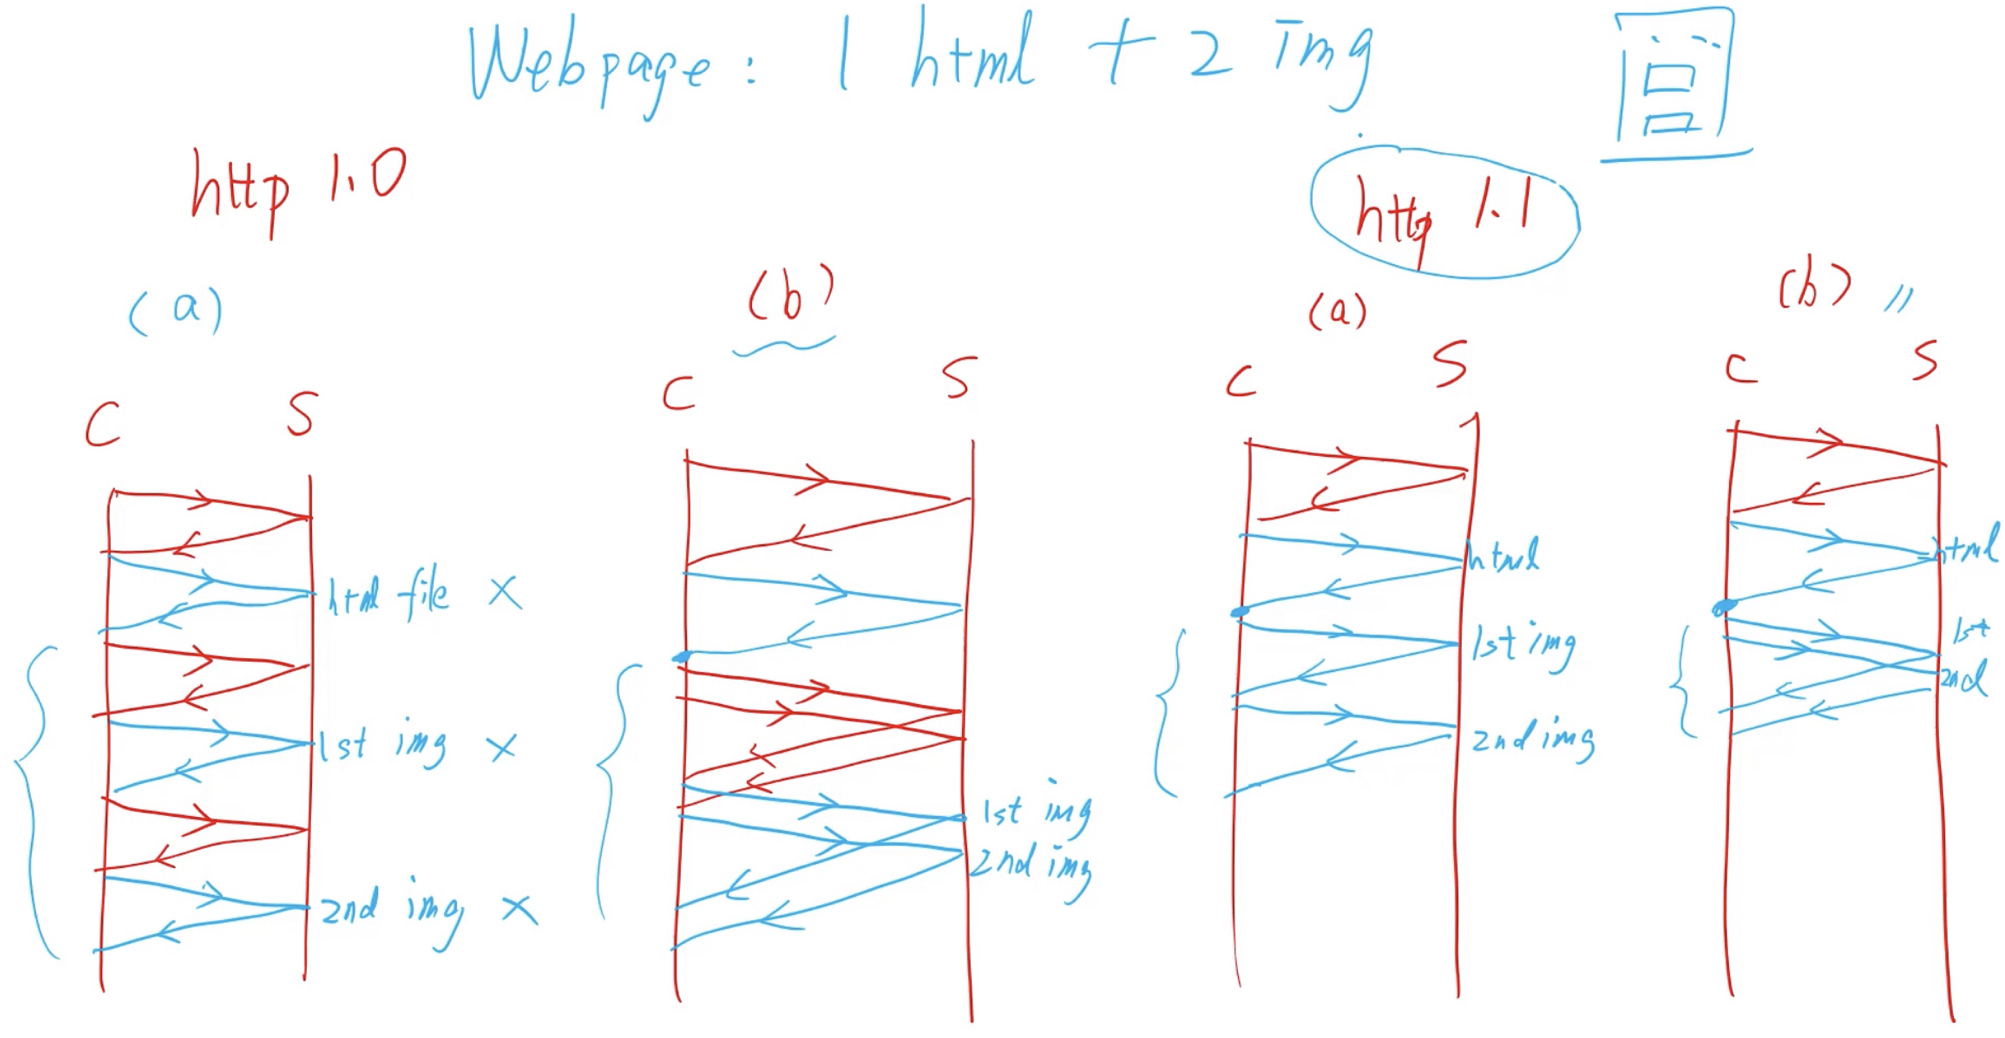
\includegraphics[scale=.12]{./assets/httpDiagrams}

		\textbf{HTTP Request}\\
		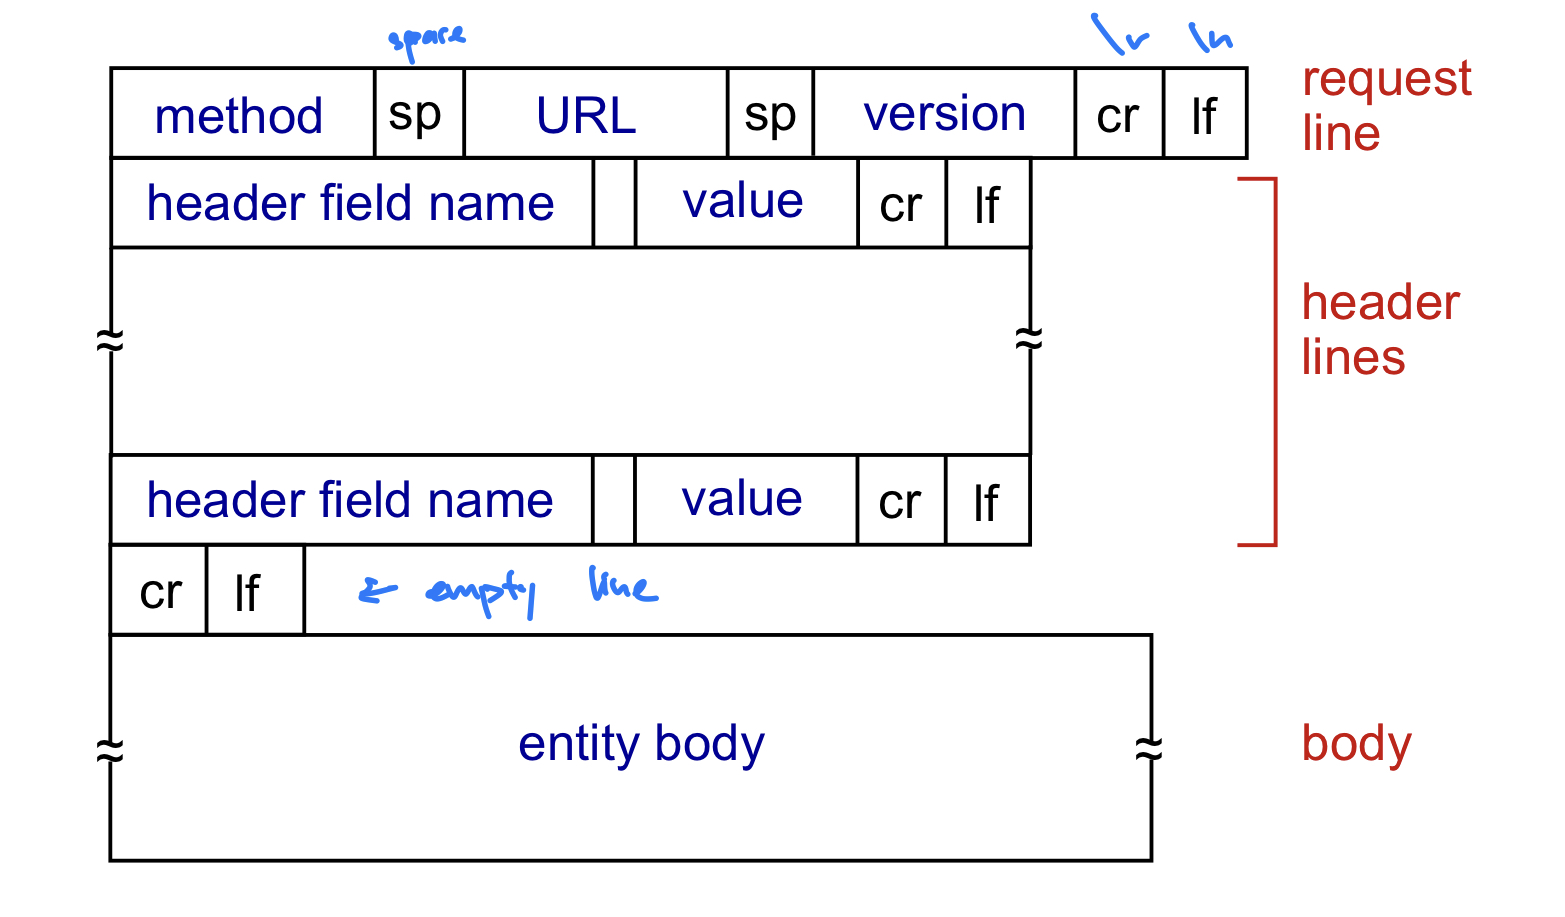
\includegraphics[scale=.14]{./assets/httpRequest}
		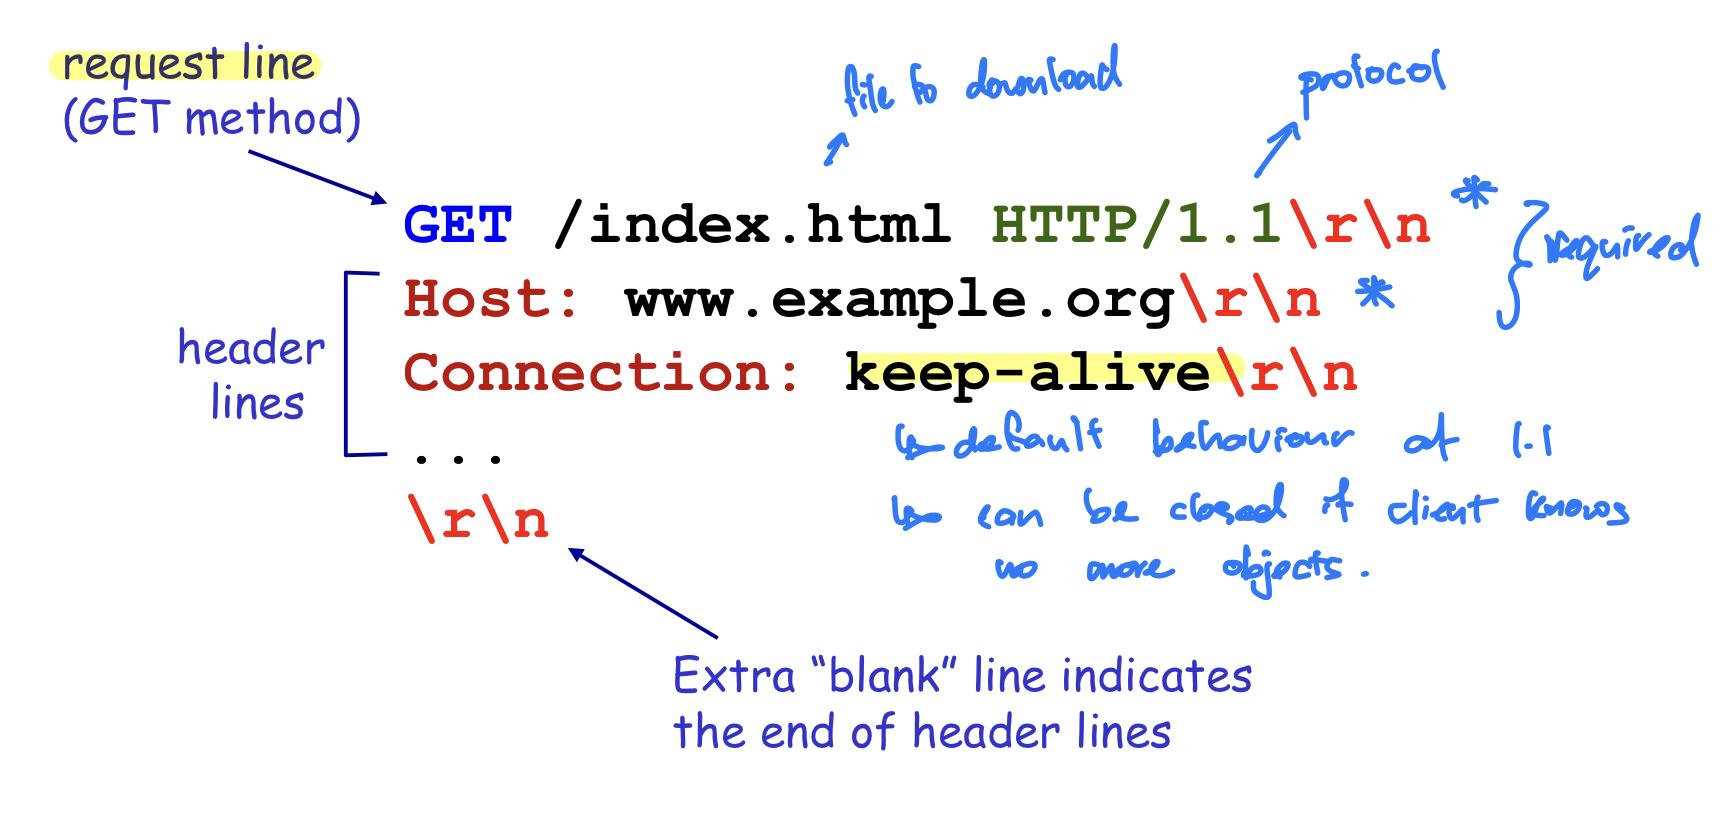
\includegraphics[scale=.12]{./assets/httpRequestEg}\\
		Request Method Types:\\
		1.0: GET, POST (upload input to server), HEAD (leave out requested object)\\
		1.1: GET, POST, HEAD, PUT (uploads file to path specified in URL field), DELETE (deletes file specified in URL field)\\

		\textbf{HTTP Response}\\
		Response Status Codes:\\
		- 200: OK\\
		- 301: Moved Permanently (new location specified later in message)\\
		- 403: Fobidden\\
		- 404: Not found\\
		- 304: Not Modified\\
		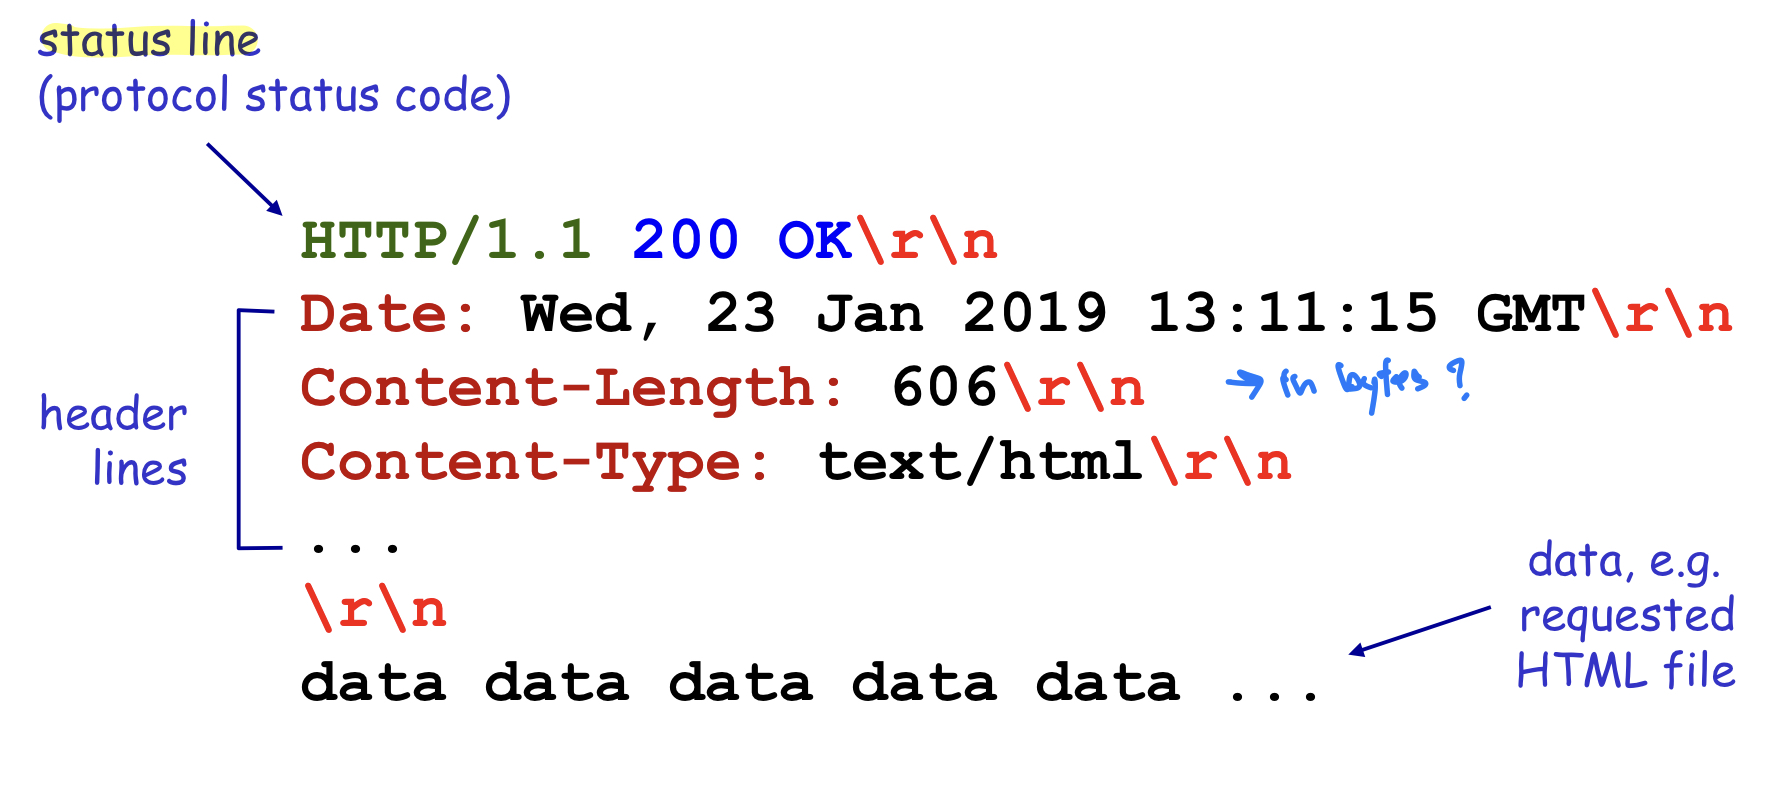
\includegraphics[scale=.12]{./assets/httpResponseEg}

		\textbf{Cookies}\\
		HTTP designed to be stateless - server maintains no information about past client requests\\
		Cookie: http messages carry state (forever, expiry, memory only)\\
		1. cookie header field of http request/ response messages\\
		2. cookie file kept on user's host, managed by user's browser\\
		3. backend database at website\\

		\textbf{Conditional Get}\\
		- Goal: don't send object if client cache has up to date cached version\\
		- cache: specify date of cached copy in http request; \texttt{If-modified-since: <date>}\\
		- server: response contains no object if cached copy is up to date; response is 304\\

		\textbf{Domain Name System}\\
		Identify host by:
		1. Hostname: eg, www.example.org\\
		2. IP address: eg, 93.184.216.34 (32-bit int)\\
		DNS translates between the two\\
		Client carries out DNS query to determine the IP address corresponding to server name prior to connection\\
		\red{NOTE}: 1 hostname could map to many IP addresses (for load balancing purposes)\\

		\textbf{DNS Resource Record (RR)}\\
		Mappings are stored as RR\\
		RR format: \texttt{(name, value, type, ttl)}\\

		Types:
		1. A - name is hostname; value is IP addr\\
		2. NS (name server) -name is domain (eg. nus.edu.sg); value is hostname of authoritative name server for domain.\\
		3. CNAME - name is alias name (eg. www.nus.edu.sg) for some canonical (real) name; value is canonical name (eg. mgnzsqc.x.incapdns.net)\\
		4. MX (mail exchanger) - value is the name of mail server associated with name\\

		\textbf{Distributed Hierarchical Databases}\\
		DNS is stored in RR in distributed databases implemented in hierarchy of many name servers\\
		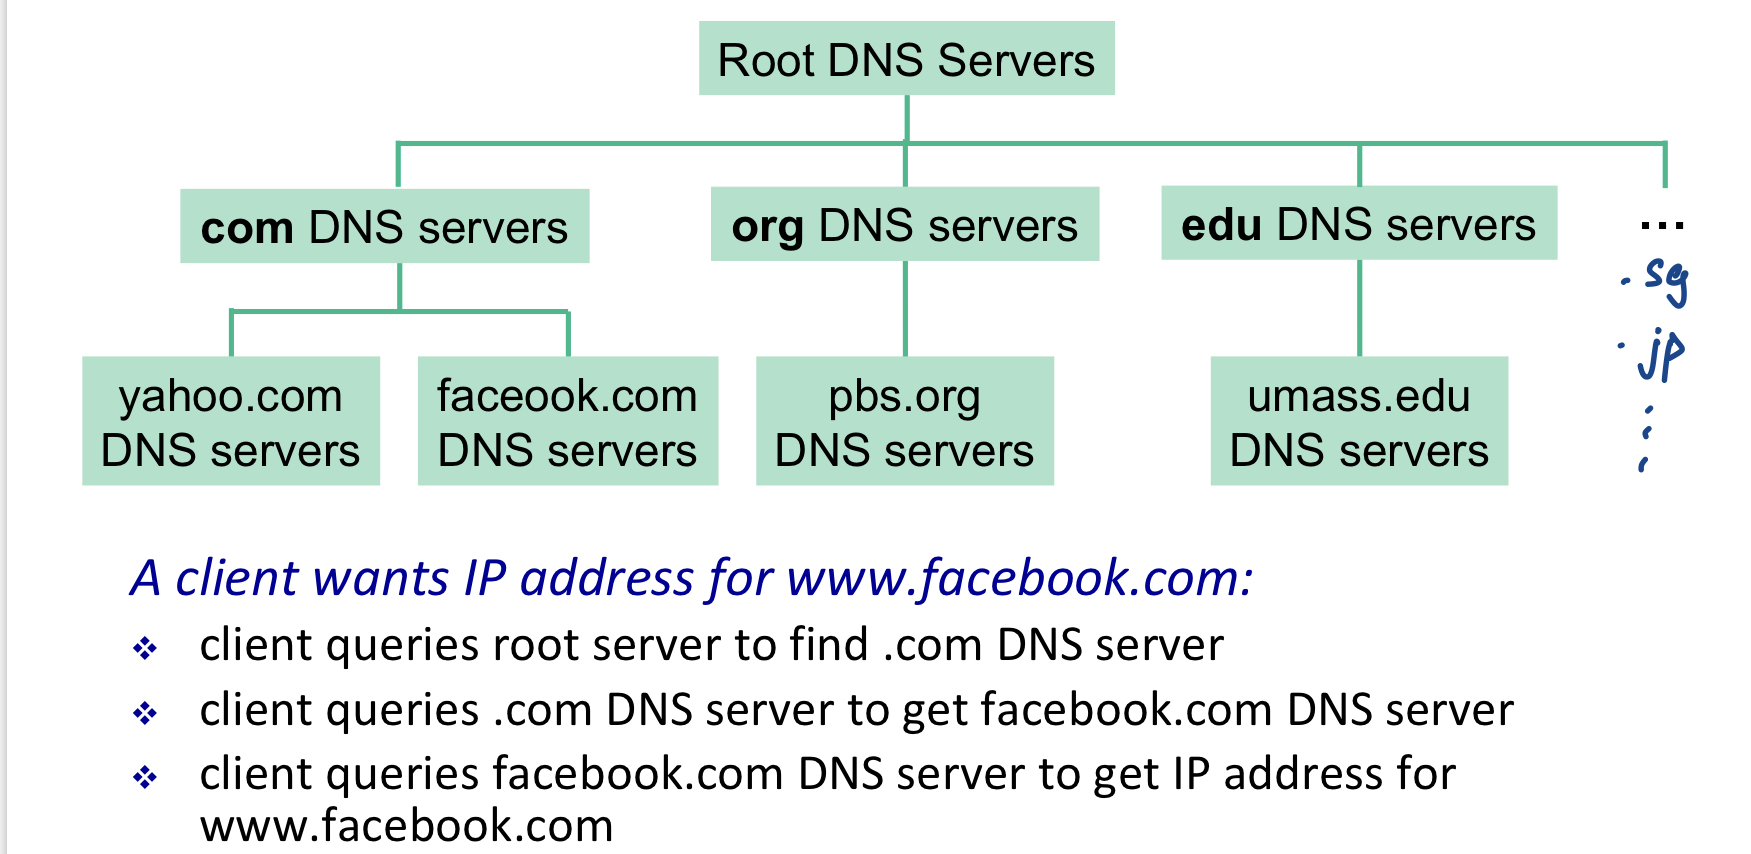
\includegraphics[scale=.13]{./assets/dnsDatabases}

		Root servers\\
		- Answers request for records in the root zone by returning a list of the authoritative NS for the appropriate top level domain (TLD)\\

		Top Level Domain\\
		- responsible for com, org, net, edu, etc and all top-level country domains, eg. sg, jp, etc.\\

		Authoritative Servers\\
		- Organisation's own DNS server(s), providing authoritative hostname to IP mappings for organisation's named hosts (eg. web, mail)\\

		\textbf{Local DNS server}\\
		- Does not strictly belong to hierarchy\\
		- Each ISP has one local DNS server (aka default name server)\\
		- When host makes DNS query, query is sent to local DNS server\\
		- Retrieve name-to-address translation from local cache\\
		- Local DNS server acts as proxy and forwards query into hierarchy if answer not found locally\\

		\textbf{DNS Caching}\\
		Caches mapping once it learns of it\\
		- may be out of date\\
		- cached entries expire after some time (TTL)\\
		- if name host changes IP address, may not be known Internet-wide until TTL expire\\
		Runs over \red{UDP}\\

		\textbf{DNS name resolution}\\
		iterative and recursive\\
		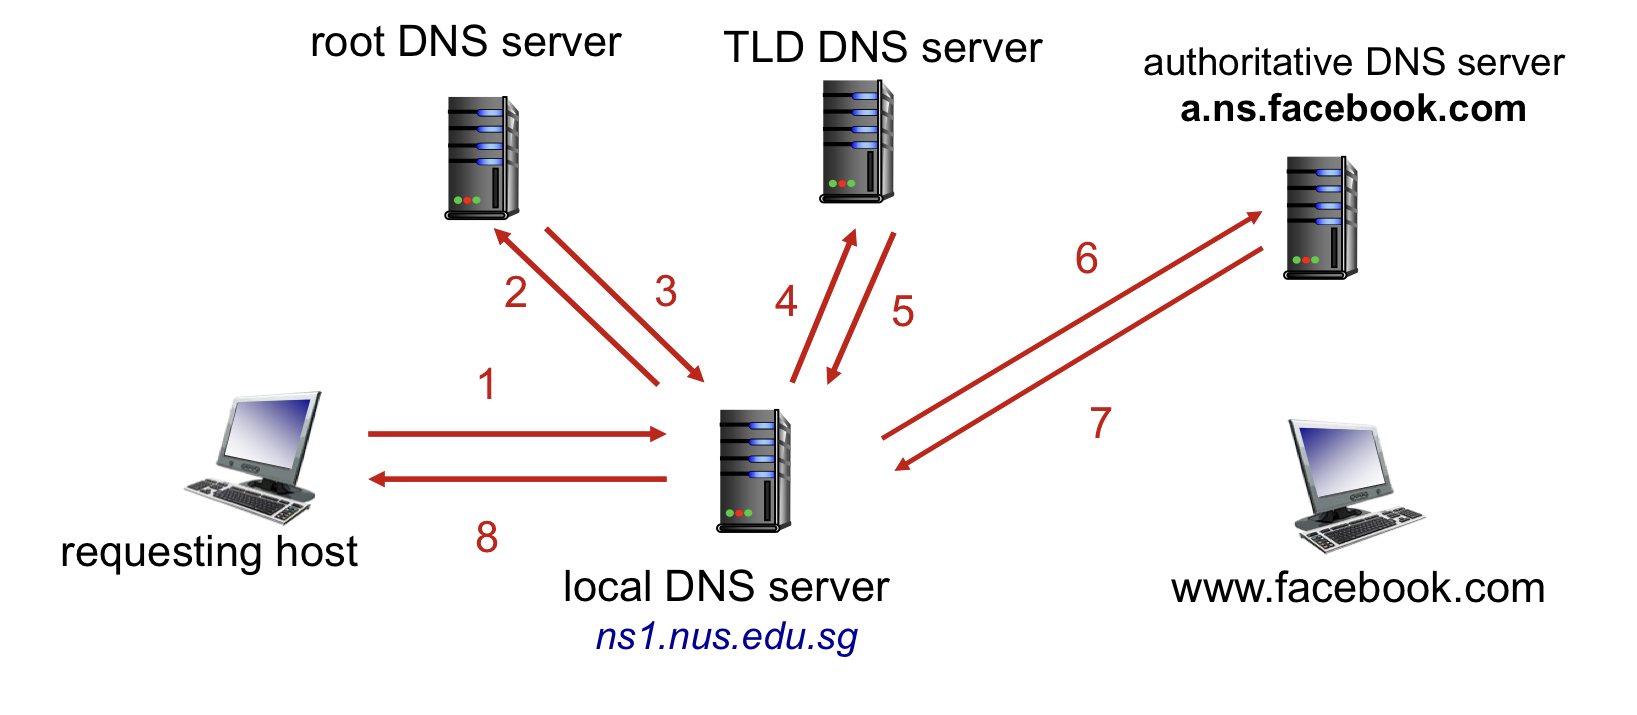
\includegraphics[scale=.12]{./assets/iterativeDns}\\
		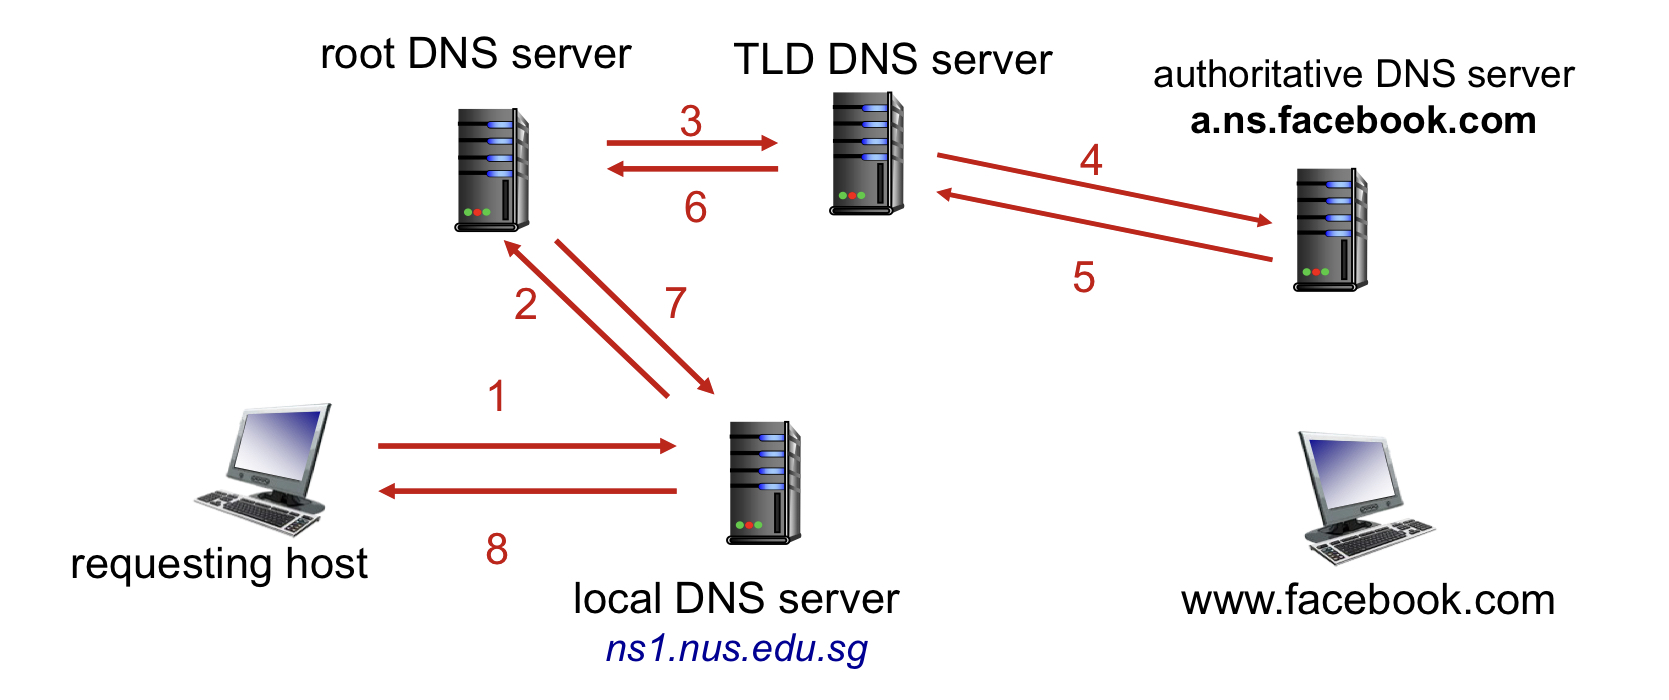
\includegraphics[scale=.12]{./assets/recursiveDns}\\
		\red{NOTE}: Recursive rarely used as servers cannot respond to other queries until it recieves an answer, eg root DNS cannot answer other queries until TLD server replies\\

		\textbf{Socket Programming}\\
		Process: program running within a host\\
		- Within host, two processes communicate using \red{inter-process communication (defined by OS)}\\
		- Processes in different hosts communicate by \red{exchanging messages (according to protocols)}\\
		- Identified by \red{(IP address, port number)} (port number is a 16 bit int, 1-1023 are reserved)\\

		\textbf{Sockets}\\
		Socket is the software interfrace between app processes and transport layer protocols
		- Process send/ receives messages to/ from its \red{socket}\\
		- Programming-wise: a set of APIs\\
		Application treat the Internet as a black box, sending and receiving messages through sockets\\

		Types of sockets:\\
		1. TCP: reliable, byte stream-oriented socket\\
		2. UDP: unreliable datagram socket\\

		\textbf{Socket Programming with \red{UDP}}\\
		\red{UDP: no connection between client and server}\\
		- Sender explicitly attaches destination IP addr and port number to \red{each packet}\\
		- Receiver extracts sender IP addr and port number from the received packet\\
		\red{1} socket listens to \red{multiple} clients.\\

		\textbf{Socket Programming with \red{TCP}}\\
		- When client creates socket, client TCP establishes a connection to server TCP\\
		- When contacted by client, server TCP \red{creates} new socket for server process to communicate with that client\\
		This allows server to talk with multiple clients individually.\\
		TCP socket pairs (?) are uniquely identified by \blue{(server IP, server port, client IP, client port)}\\

		TCP socket vs UDP socket\\
		- TCP: two processes communicate as if there is a ``pipe'' between them. Send data $\rightarrow$ write data to pipe, \blue{no need to attach} dest IP and port to each packet. Pipe is there until one of the two processes closes it. Pipe is also \blue{reliable}\\
		- UDP: Form UDP packet explicitly and \blue{attach} dest IP and port no to every packet.\\







		
		
		
		
	\end{multicols*}
\end{document}
